\documentclass[9pt,twocolumn,twoside]{../../styles/osajnl}
\usepackage{fancyvrb}
\journal{i524} 

\title{CoreOS}

\author[1, *]{Ribka Rufael}


\affil[1]{School of Informatics and Computing, Bloomington, IN 47408, U.S.A.}


\affil[*]{Corresponding authors: rrufael@umail.iu.edu HID: S17-IO-3016}

\dates{paper-001, February 25, 2017}

\ociscodes{CoreOS, Container, cloud, Linux}

% replace this with your url in github/gitlab
\doi{\url{https://github.com/cloudmesh/sp17-i524/raw/master/paper1/S17-IO-3016/report.pdf}}


\begin{abstract}

  CoreOS is a minimal Linux operating system that allows application
  to run on containers. CoreOS can be used on clouds from EC2,
  Rackspace, GCE or virtual machines such as Vagrant, VMware,
  OpenStack or on physical servers such as PXE, iPXE, ISO. CoreOS
  makes use of it's disk partions to achieve continous updates to the
  operating system without manual interaction. In CoreOS service
  discovery is achieved by etcd, applications are run on Docker and
  process management is achieved by fleet.  
\newline
\end{abstract}

\setboolean{displaycopyright}{true}

\begin{document}

\maketitle

\section{Introduction}

CoreOS also known as CoreOS Container Linux is a light weight Linux
operating system that is designed to be used for container
infrastructure. CoreOS allows applications to run on containers so
that there is abstraction layer between applications and the operating
system. The separation of applications and operating system helps
avoid dependencies.  CoreOS can be run on clouds, virtual or physical
servers. CoreOS allows the ability for automatic software updates in
order to make sure containers in cluster are secure and reliable. It
also makes managing large cluster environments easier. One of the
differences between CoreOS Linux and traditional Linux distribution is
that, in the case of traditional Linux distribution operating system,
utilities(such as systemd) and software(such as Python and Java) are
put together but in the case of CoreOS Linux only operating system and
utilities are bundled together. In CoreOS Linux applications and
software(such as Python and Java) are run on containers as shown in
Figure 1 \cite{www-core}.


\begin{figure}[htbp]
\centering
\fbox{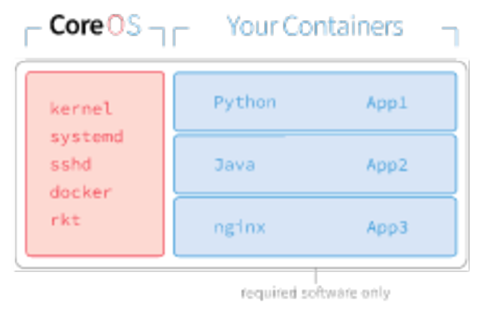
\includegraphics[scale=0.75]{images/CoreOS}}
\caption{CoreOS container layout  \cite{www-core}. }
\label{fig:false-color}
\end{figure}

CoreOS is an open source software that is provided by CoreOS,
Inc. CoreOS, Inc also provides open source tools like etcd, rkt and
flannel. CoreOS, Inc also has commercial products Kubernetes and
CoreOS stack. These products can be used on top of CoreOS for
additional functionalities like for example Kubernetes can be used for
orchestration and management of containers that run on CoreOS
\cite{www-core}.

Since CoreOS Linux is designed to be used in container frameworks, it
makes it one of the candidates to be included into big data projects
software stack that has container cluster infrastructure. Containers
are multiple instances that contain applications and the softwares
needed to run these applications sharing the same underlying operating
system \cite{julian2016containers}. Big data projects in science or
business involve processing of large amount of data.  These big data
projects are hosted on bare metal servers which are dedicated physical
servers that are only used by one tenant or on clouds. Big data
projects in science and in business sector can benefit from container
frameworks that provide flexibility, ease of deployment, adding or
removing container clusters based on demand
\cite{julian2016containers}.

\section{CoreOS Architecture and Installation}

CoreOS has 9 disk partitions. CoreOS makes use of these partions to
achieve continous updates to the operating system. Having this disk
layout aslo allows CoreOS to be able to reverse the updates in the
event of unsuccessful updates. The disk partions are: 1) EFI-SYSTEM
which contains the bootloader and the partition type is VFAT. 2)
BIOS-BOOT, ROOT-C and the 7th partion these partions have no partion
format and are reserved for future use. 3) USR-A and USR- B are the
active and passive partions that container linux sits on. Only one of
them can be active at a time and partion type is EXT4 depending on
which one is active. 4) OEM has EXT4 as partition type and this is
where OEM platform related configurations like custom networking and
running an agent are stored. 5) OEM-CONFIG serves as an alternative
place for an OEM. 6) ROOT may have EXT4, BTRFS, or XFS as partion type
and it is used for keeping data which is persistent and this partion
is stateful \cite{www-core}.

CoreOS Linux comes bundled with etcd, fleet and Docker. In CoreOS
Container Linux service discovery is achieved by etcd, applications
are run on Docker and process management is achieved by fleet. Service
discovery in CoreOS Linux is achieved by etcd. Key value store on etcd
is distributed and stored on all machines that run CoreOS Linux.
State and configuration of each container running on CoreOS is stored
in etcd key value store and this information is used to identify which
container is selected to receive service requests. This service
discovery capability makes it easy to add or remove machines. There is
a command line interface that comes preinstalled on CoreOS linux
called etcdctl that can be used to change and get key value data from
etcd using etcdctl set and etcdctl get respectively. Another command
that can be used for setting and reading key value is curl
\cite{www-coreOSquickstart}.

Container management in CoreOS linux is made possible by Docker.  All
applications run on Docker. Containers can be launched using Docker's
command line interface \cite{www-coreOSquickstart}.

the third component of CoreOS is fleet and it is used for management
of containers with Docker installed. fleet is init system. init system
is a process that gets started before any other process when a machine
boots and runs till the machine is shutdown. fleet has fleetctl a
command line interface that can be used to check the status of
containers, to start containers and to stop containers
\cite{www-coreOSquickstart, www-wiki}.

There is no package manager for installing, upgrading, configuring
softwares in CoreOS. Softwares are installed as containers in CoreOS
Linux operating system. In order to apply updates, CoreOS makes use of
two root partitions one is active and the other is passive.First the
updates to CoreOS are applied to passive partion and upon reboot all
the updates are applied to the active partition \cite{coreOSBook}.

CoreOS can be installed on clouds from EC2, Rackspace, GCE or virtual
machines such as Vagrant, VMware, OpenStack or on physical servers
such as PXE, iPXE, ISO \cite{www-coreOSquickstart}. Based on the
information provided on CoreOS site, CoreOS container can be setup
using Vagrant. Vagrant, virtual machine manager, can be used to run
CoreOS on a single machine with Windows, OS X or Linux operating
systems. It is recommened to have Vagrant version 1.6.3 or
latest. Virtual machines by VirtualBox or VMware are both supported by
Vagrant \cite{www-coreOSvagrant}.

\section{Licensing}

CoreOS Container Linux is an open source operating system . It is
comprised of other programs and documents developed by other
individuals and companies. All original components that are part of
CoreOS Container Linux are licensed under Apache 2.0. At the time of
writing is paper, the latest version of CoreOS Container Linux is
1325.1.0 \cite{www-core}.


\section{Performance}

In a study done by Purdue University, performance tests between CoreOS
899.5.0 on Docker and Red Hat Enterprise Linux 6.5 were performed. In
their study, the tests were run on 24-core AMD Opteron systems, with
2.1 GHz processors, 48 GB memory and 10Gbps Ethernet connection.  For
HPL performance tests, the native RHEL 6.5 system with performance
measurement of 7.839 GFLOPS performed slower than the container
environment with CoreOS on Docker with performance measurement of
7.811 GFLOPS. For the network throughput measurement iperf was
used. The results for RHEL 6.5 system were 8.26 Gbps for upload
throughput and 9.38 Gbps for download throughput. The result for
container environment with CoreOS on Docker were 8.43 Gbps for upload
throughput and 9.37 Gbps for download throughput. Network File System
throughput was done using iozone and results are shown in Figure 2
\cite{julian2016containers}.

\begin{figure}[htbp]
\centering
\fbox{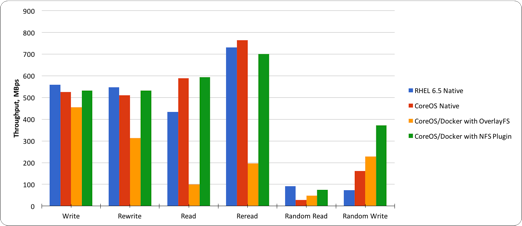
\includegraphics[width=\linewidth]{images/File-server-throughput}}
\caption{File Server throughput \cite{julian2016containers}. }
\label{fig:false-color}
\end{figure}

In another study done in Institute of Informatics – Federal University
of Rio Grande do Sul, performance analysis of ClickOS, CoreOS and
OS\textsuperscript{v} was performed. Network Functions
Virtualization(NFV) allows virtualization of network services such as
firewalls and DNS. In their paper comparison of ClickOS, CoreOS and
OS\textsuperscript{v} as NFV based tools was performed. They compared
boot time, response time and memory consumption for the three
virtualization technologies. As per their evaluation result, ClickOS
has the lowest boot time and response time followed by CoreOS and with
regards to memory consumption, CoreOS has the smallest memory usage
followed by ClickOS. Based on the result OS\textsuperscript{v} has the
slowest boot time and response time as compared to CoreOS and
ClickOS. Also for memory consumption, OS\textsuperscript{v} has the
highest cosumption as compared to the other two technologies used
\cite{2016NFVSolutions}.

\section{Use Cases}

In this section use cases from big data and other areas where CoreOS
Linux is used are discussed.

\subsection{Use Cases  for Big Data}

Metagenomics RAST server(MG-RAST) is free access portal that can be
used by researchers who study microbes for accessing and analyzing
metagenomics data(Random community genomes)
\cite{meyer2008metagenomics}. CoreOS Container Linux and fleet are
the technologies used on MG-RAST container application
servers. Researchers can input data into MG-RAST portal through
script, web site or REST API \cite{wilke2016mg}.

\subsection{Other Use Cases}

CoreOS Container Linux on Amazon EC2 cloud was used to implement the
project Two-stage Stochastic Programming Resource Allocator
(2SPRA). The language used to implement was Python. In this
project, they tried to address the problem that exist in most data
centers of over provisioning resources in order to achieve performance
service level objective. 2SPRA is a resource allocation scheme and it
is able to optimize resource allocation for containerized web services
based on varying workloads. 2SPRA analyzes the relationship between
change in workload, resource allocation and response latency in order
to calculate the the number of containers needed. In this experimental
work, CoreOS was used inorder to simulate real word scenarios of n
tier application servers running on containers. The test architecture
has client Java based emulator which creates multiple user sessions at
the same time, web hosting platform with where RUBis benchmark is
installed on Virtual machine with CoreOS version stable r717.3.0 and
the third component is 2SPRA implemented in Python running on Virtual
machine \cite{2SPRA}.


\section{Educational material} 

CoreOS website contains detailed documentations and materials for
anyone who is interested in setting up CoreOS Container Linux on
clouds, virtual or physical servers \cite{www-coreOSquickstart}.
Users who are interested can contribute to the CoreOS open source
projects through GitHub \cite {www-coregit}.

The book titled CoreOS Essentials, also has information about CoreOS
overview and its installation \cite{coreOSBook}.

\section{Conclusion} 
CoreOS Linux is a light weight Linux based operating system that is
designed for containers. It provides abstraction by separating the
operating system from application and softwares. Operating system
updates to CoreOS are automatic without a need for user
interaction. CoreOS can be installed on clouds from EC2, Rackspace,
GCE or virtual machines such as Vagrant, VMware, OpenStack or on
physical servers such as PXE, iPXE, ISO.  

CoreOS Linux aims to make applications and microservices running on
containers secure, easy to deploy and portable. Big data projects can
leverage these benefits that come with CoreOS Linux by adding it to
their infrastructure.

As previous performance results have shown, CoreOS Linux has the lowest
memory usage compared to other operating systems namely ClickOS and
OS\textsuperscript{v} \cite{2016NFVSolutions}.


\section*{Acknowledgements}
The author would like to thank Professor Gregor von Laszewski and
associate instructors for their help and guidance.



% Bibliography

\bibliography{references}
 

\newpage

\appendix



\end{document}
